\phant{CƠ SỞ LÝ THUYẾT}\label{sec:coso}

\subsection{Tập Mandelbrot}

\subsubsection{Định nghĩa và thuật toán thoát}

Tập Mandelbrot được định nghĩa từ phép lặp trên mặt phẳng phức. Với mỗi số phức
$c\in\mathbb{C}$, xét dãy
\begin{equation}
  z_0 = 0, \qquad z_{n+1} = z_n^2 + c, \quad n=0,1,2,\ldots
  \label{eq:mandel}
\end{equation}
Điểm $c$ thuộc tập Mandelbrot nếu dãy $(z_n)$ bị chặn. Người ta chứng minh được
rằng nếu tồn tại $n$ sao cho $|z_n|>2$ thì dãy phân kỳ ra vô cùng; do đó điều kiện
thoát thực dụng là $|z_n|>R$ với bán kính thoát $R=2$. Trong thực hành, số vòng
lặp bị chặn trên bởi $I_{\max}$; điểm nào không thoát sau $I_{\max}$ vòng được coi
là thuộc tập (hoặc nằm sát tập) và thường được tô màu đen.

Với mỗi điểm ảnh, tọa độ phức được ánh xạ tuyến tính từ chỉ số điểm ảnh:
\begin{equation}
  c = \bigl(c_{\mathrm{real}} + (x - W/2)\,s/W\bigr)
      + i\bigl(c_{\mathrm{imag}} + (y - H/2)\,s/H\bigr),
\end{equation}
trong đó $W,H$ là kích thước ảnh, $s$ là tỉ lệ khung nhìn, và
$(c_{\mathrm{real}},c_{\mathrm{imag}})$ là tâm. Cấu hình mặc định của bài báo là
$I_{\max}=1000$, $c=-0{,}75+0i$, $s=3{,}0$ và ảnh $1920\times1080$ điểm ảnh
\cite{diehl2026}. Hình~\ref{fig:mandel} minh họa kết quả do hai chương trình
khác nhau sinh ra.

\begin{figure}[H]
  \centering
  \begin{minipage}[t]{0.48\textwidth}
    \centering
    
\includegraphics[width=\linewidth]{figures/mandelbrot_coroutine.png}\\[2pt]
    {\small (a) Mã coroutine}
  \end{minipage}\hfill
  \begin{minipage}[t]{0.48\textwidth}
    \centering
    
\includegraphics[width=\linewidth]{figures/mandelbrot_mpi.jpg}\\[2pt]
    {\small (b) Mã MPI+OpenMP của ChatGPT-5}
  \end{minipage}
  \caption{Tập Mandelbrot với 1000 vòng lặp, tỉ lệ 3,0, tâm $(-0{,}75;0)$.
  Cùng một mô hình có thể sinh hàm tô màu khác nhau cho bản bộ nhớ chia sẻ và
  bản bộ nhớ phân tán. Nguồn: bài báo \cite{diehl2026}.}
  \label{fig:mandel}
\end{figure}

Mã giả của phép tính một điểm ảnh như sau:

\begin{lstlisting}[language=C++,caption={Tính số vòng lặp thoát cho một điểm ảnh.},label={lst:escape},numbers=none]
int escape(double cr, double ci, int max_iter) {
    double zr = 0.0, zi = 0.0;
    int n = 0;
    while (n < max_iter && zr*zr + zi*zi <= 4.0) {
        double t = zr*zr - zi*zi + cr;   // phan thuc cua z^2 + c
        zi = 2.0*zr*zi + ci;             // phan ao
        zr = t;
        ++n;
    }
    return n;
}
\end{lstlisting}

Độ phức tạp tuần tự là $\mathcal{O}(W\cdot H\cdot I_{\max})$ trong trường hợp xấu
nhất. Trên thực tế, phần lớn điểm ảnh nằm ngoài tập thoát chỉ sau vài vòng lặp,
trong khi các điểm sát biên hoặc nằm trong tập tiêu tốn đủ $I_{\max}$ vòng. Sự
chênh lệch này tạo ra \term{mất cân bằng tải} tự nhiên, là đặc trưng quan trọng
khi đánh giá các chiến lược chia việc.

\subsubsection{Tính chất song song hiển nhiên}

Giá trị của mỗi điểm ảnh chỉ phụ thuộc vào tọa độ của nó và các tham số toàn cục;
không có phụ thuộc dữ liệu giữa các điểm ảnh. Vì vậy, miền tính toán có thể chia
tùy ý cho các luồng hoặc tiến trình mà không cần đồng bộ trong pha tính. Đây là
lý do bài toán được gọi là song song hiển nhiên. Hệ quả là:

\begin{itemize}
  \item Không có tranh chấp dữ liệu trong pha tính; mỗi đơn vị ghi vào một vùng
        ảnh riêng.
  \item Chi phí phụ trội chủ yếu đến từ khởi tạo luồng, lập lịch vòng lặp, ghi
        ảnh và — với MPI — truyền thông gom kết quả.
  \item Hiệu năng phụ thuộc mạnh vào cân bằng tải: chia tĩnh theo hàng có thể
        lệch nếu một dải chứa nhiều điểm biên.
\end{itemize}

Chính vì cấu trúc đơn giản, bài toán này là phép thử tốt để quan sát \emph{cách}
LLM biểu diễn song song, thay vì bị che khuất bởi độ phức tạp của thuật toán.
Nếu mã sinh ra không mở rộng trên một bài toán song song hiển nhiên, nguyên nhân
gần như chắc chắn nằm ở tầng điều khiển luồng, tầng thư viện hoặc tầng đo đạc.

\subsubsection{Định dạng đầu ra PBM và PGM}

Bài báo yêu cầu xuất ảnh ở định dạng PBM để kiểm tra tính đúng mà không cần thư
viện ngoài. Cần phân biệt chính xác các biến thể của họ Netpbm:

\begin{itemize}
  \item \textbf{P1}: bitmap ASCII, mỗi điểm ảnh là ký tự \code{0} hoặc \code{1}.
  \item \textbf{P4}: bitmap nhị phân, mỗi byte chứa 8 điểm ảnh đơn sắc.
  \item \textbf{P2}: ảnh xám ASCII, mỗi điểm ảnh là một số nguyên.
  \item \textbf{P5}: ảnh xám nhị phân, mỗi điểm ảnh là một byte (0--255).
\end{itemize}

PBM đúng nghĩa chỉ gồm P1 và P4; P2/P5 thuộc PGM. Bài báo dùng cụm “PBM” theo
nghĩa rộng của họ Netpbm. Sự nhập nhằng này không chỉ là vấn đề thuật ngữ: nó
trực tiếp tạo ra một lớp lỗi quan sát được, khi mã tính màu theo thang 256 mức
(P5) nhưng lại ghi header và dữ liệu theo định dạng 1 bit (P4), dẫn tới ảnh đen
hoặc ảnh sai định dạng \cite{diehl2026}. Phần~\ref{sec:ketqua} phân tích lỗi này
chi tiết.

\subsection{Lập trình song song trong C++ hiện đại}

C++ không có một mô hình song song duy nhất; qua từng phiên bản chuẩn, ngôn ngữ bổ
sung những mức trừu tượng khác nhau. Hình~\ref{fig:timeline} tóm tắt dòng thời
gian. Điểm quan trọng là các cơ chế này không tương đương nhau về ngữ nghĩa, chi
phí và khả năng kiểm soát tài nguyên, nên cùng một prompt có thể dẫn tới những
chương trình rất khác nhau.

\begin{figure}[H]
  \centering
  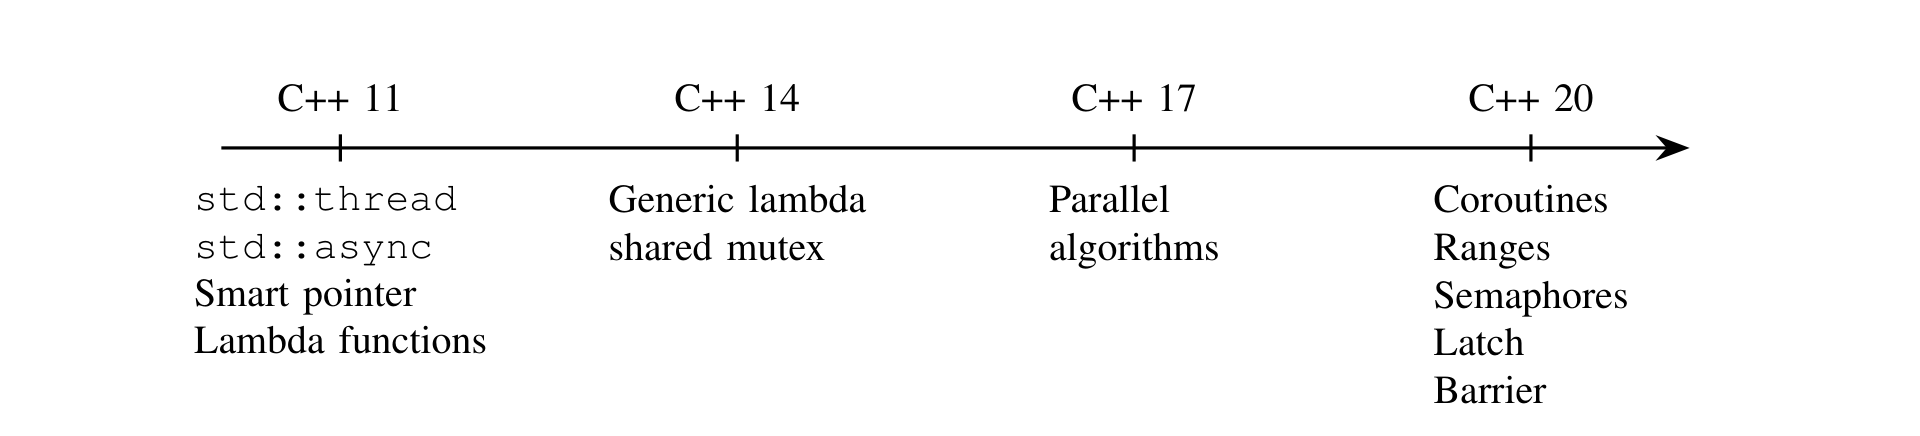
\includegraphics[width=0.95\textwidth]{figures/fig_timeline.png}
  \caption{Dòng thời gian các tính năng song song được bổ sung vào chuẩn C++.
  Nguồn: bài báo \cite{diehl2026}, phỏng theo \cite{diehl2023shared}.}
  \label{fig:timeline}
\end{figure}

\subsubsection{C++11: luồng và lập trình bất đồng bộ}

C++11 đưa vào \code{std::thread}, \code{std::async}, \code{std::future},
\code{std::promise}, lambda và con trỏ thông minh. Trong mô hình bất đồng bộ,
một hàm hoặc lambda được chạy trên một luồng riêng; kết quả được chuyển về qua
đối tượng \code{std::future<T>}. Lời gọi \code{future.get()} sẽ chờ đến khi kết
quả sẵn sàng và trả về giá trị, hoặc ném lại ngoại lệ đã xảy ra trong luồng bất
đồng bộ.

\begin{lstlisting}[language=C++,caption={Mẫu bất đồng bộ với \code{std::async} và \code{std::future}.},label={lst:async}]
std::vector<std::future<void>> tasks;
for (int t = 0; t < nthreads; ++t)
    tasks.push_back(std::async(std::launch::async,
        [&, t] { render_rows(t, nthreads); }));
for (auto& f : tasks) f.get();   // cho tat ca hoan thanh
\end{lstlisting}

Ba đặc điểm cần lưu ý. Thứ nhất, \code{std::async} không bảo đảm mỗi tác vụ có
một luồng riêng; nó có thể dùng thread pool hoặc trì hoãn (\code{launch::deferred}).
Thứ hai, hủy một \code{std::future} từ \code{std::async} có thể chặn cho tới khi
tác vụ kết thúc, nên vòng đời đối tượng quan trọng hơn tưởng tượng. Thứ ba, C++11
không cung cấp API chuẩn để đặt số luồng toàn cục; việc điều khiển số luồng phụ
thuộc hoàn toàn vào cách người lập trình chia tác vụ.

\subsubsection{C++17: thuật toán song song}

C++17 mở rộng thư viện thuật toán bằng execution policy trong header
\code{<execution>}:
\begin{itemize}
  \item \code{std::execution::seq} — thực thi tuần tự;
  \item \code{std::execution::par} — thực thi song song;
  \item \code{std::execution::par\_unseq} — song song, cho phép vector hóa.
\end{itemize}
Ví dụ, \code{std::transform(std::execution::par, ...)}
cho phép thư viện tự chia vòng lặp cho nhiều luồng.

Điểm cốt lõi — và cũng là nguồn lỗi chính trong bài báo — là chuẩn C++ \emph{không}
quy định cách hiện thực execution policy. Với GCC/libstdc++, backend mặc định cho
thuật toán song song là Intel TBB, không phải OpenMP. Do đó, biến môi trường
\code{OMP\_NUM\_THREADS} không điều khiển được số luồng của
\code{std::execution::par}. Muốn giới hạn số luồng, phải dùng API riêng của TBB,
chẳng hạn \code{tbb::global\_control}. Đây là kiến thức hệ sinh thái không suy ra
được từ tài liệu chuẩn C++.

\begin{lstlisting}[language=C++,caption={Thuật toán song song C++17 và giới hạn số luồng bằng TBB.},label={lst:par}]
#include <execution>
#include <algorithm>
#include <tbb/global_control.h>

tbb::global_control limit(tbb::global_control::max_allowed_parallelism, nthreads);
std::for_each(std::execution::par, pixels.begin(), pixels.end(),
              [&](Pixel& p) { p.iter = escape(p.cr, p.ci, max_iter); });
\end{lstlisting}

\subsubsection{C++20: coroutine}

Coroutine C++20 là hàm có thể tạm dừng và tiếp tục tại các điểm xác định, không
cần một ngăn xếp riêng cho mỗi lần dừng (\term{stackless}). Ngôn ngữ chỉ cung cấp
ba từ khóa \code{co\_await}, \code{co\_yield}, \code{co\_return}; phần còn lại do
người lập trình định nghĩa: kiểu \code{task}, \code{promise\_type}, scheduler và
cách quản lý vòng đời.

Trình biên dịch biến đổi thân hàm coroutine thành một máy trạng thái. Mỗi lần gọi
tạo ra một \term{coroutine frame} chứa tham số, biến cục bộ và trạng thái tạm
dừng. Đối tượng \code{promise\_type} điều khiển hành vi:

\begin{itemize}
  \item \code{initial\_suspend()}: coroutine dừng ngay khi được gọi hay chạy luôn.
  \item \code{return\_void()} hoặc \code{return\_value(v)}: tương ứng với
        \code{co\_return;} hoặc \code{co\_return v;}.
  \item \code{yield\_value(v)}: tương ứng với \code{co\_yield v;}.
  \item \code{final\_suspend()}: quyết định điều gì xảy ra khi coroutine kết thúc.
  \item \code{unhandled\_exception()}: xử lý ngoại lệ thoát ra khỏi coroutine.
\end{itemize}

Hàm \code{std::coroutine\_handle<>::done()} chỉ trả về \code{true} khi coroutine
đã dừng tại điểm \code{final\_suspend} và đang ở trạng thái treo. Nếu
\code{final\_suspend()} trả về \code{std::suspend\_never}, coroutine tự hủy frame
ngay khi kết thúc; trạng thái “đã xong” có thể không bao giờ quan sát được qua
\code{done()}. Vòng lặp chờ trong Listing~\ref{lst:corobug} vì thế có thể chạy
mãi.

\begin{lstlisting}[language=C++,caption={Vòng lặp chờ \code{done()} không bao giờ kết thúc khi \code{final\_suspend} là \code{suspend\_never}.},label={lst:corobug}]
while (!tasks[i].done()) {
    std::this_thread::yield();
}
\end{lstlisting}

Một coroutine còn có yêu cầu về quyền sở hữu: frame phải được hủy đúng một lần.
Nếu cả cơ chế \code{final\_suspend} lẫn hàm hủy của đối tượng \code{task} đều
giải phóng cùng một work item, chương trình sẽ gặp lỗi giải phóng bộ nhớ hai lần
— thường biểu hiện thành segmentation fault hoặc thông báo
\code{free(): invalid pointer}. Đây là lớp lỗi ngữ nghĩa không thể phát hiện bằng
trình biên dịch.

\subsubsection{So sánh bốn cơ chế}

Bảng~\ref{tab:cppmodels} tóm tắt khác biệt giữa bốn cách biểu diễn song song
trong C++. Cột “kiểm soát số luồng” đặc biệt quan trọng cho thực nghiệm, vì yêu
cầu cấu hình số luồng bằng dòng lệnh là một ràng buộc phi chức năng của prompt.

\begin{table}[H]
\centering
\small
\caption{So sánh các cơ chế song song bộ nhớ chia sẻ trong C++.}
\label{tab:cppmodels}
\begin{tabularx}{\textwidth}{@{}p{2.9cm} p{3.0cm} X p{2.6cm}@{}}
\toprule
\textbf{Cơ chế} & \textbf{Trừu tượng} & \textbf{Đặc điểm và rủi ro} & \textbf{Kiểm soát số luồng} \\
\midrule
C++11 async & Tác vụ và future & Dễ diễn đạt, nhưng vòng đời future và chính sách khởi chạy phức tạp; không có API chuẩn đặt số luồng & Do người lập trình tự chia tác vụ \\
C++17 parallel algorithms & Vòng lặp song song khai báo & Ngắn gọn; hành vi phụ thuộc backend (TBB với GCC); khó kiểm soát lập lịch và số luồng & Qua API backend, không qua chuẩn \\
C++20 coroutines & Tác vụ hợp tác & Linh hoạt nhất nhưng phải tự viết task, promise và scheduler; lỗi vòng đời khó thấy & Do scheduler tự xây dựng \\
OpenMP & Chỉ thị chia vòng lặp & Quen thuộc, hỗ trợ schedule; dễ sai chia sẻ dữ liệu và dễ bỏ qua số luồng & Trực tiếp qua clause hoặc biến môi trường \\
\bottomrule
\end{tabularx}
\end{table}

\subsection{OpenMP}

OpenMP là mô hình lập trình dựa trên chỉ thị (directive-based) cho bộ nhớ chia sẻ.
Mô hình thực thi là fork--join: một luồng chính tạo ra một nhóm luồng tại vùng
song song, các luồng chia việc theo vòng lặp hoặc vùng tác vụ, rồi hội tụ ở cuối
vùng. Với bài toán Mandelbrot, dạng phổ biến là:

\begin{lstlisting}[language=C++,caption={Song song hóa vòng lặp điểm ảnh bằng OpenMP.},label={lst:omp}]
#pragma omp parallel for schedule(static) num_threads(nthreads)
for (int y = 0; y < height; ++y) {
    for (int x = 0; x < width; ++x)
        image[y*width + x] = escape(...);
}
\end{lstlisting}

Số luồng có thể được đặt theo thứ tự ưu tiên sau (giảm dần):
\begin{enumerate}
  \item clause \code{num\_threads};
  \item lời gọi \code{omp\_set\_num\_threads()};
  \item biến môi trường \code{OMP\_NUM\_THREADS};
  \item giá trị mặc định của runtime.
\end{enumerate}
Việc hiểu đúng thứ tự này rất quan trọng khi kiểm tra
xem chương trình có thực sự tôn trọng tham số dòng lệnh hay không. Ngoài ra,
\code{schedule(static)} chia vòng lặp thành các khối đều nhau, trong khi
\code{schedule(dynamic)} cân bằng tải tốt hơn cho Mandelbrot nhưng tăng chi phí
lập lịch; \code{guided} là dung hòa giữa hai cách.

Một hiện tượng cần lưu ý là \term{chia sẻ giả} (false sharing): hai luồng ghi vào
các biến khác nhau nhưng cùng một dòng cache, khiến cache line bị vô hiệu hóa qua
lại. Với ảnh lớn, hiện tượng này thường không đáng kể vì mỗi luồng ghi vào vùng
nhớ cách xa nhau, nhưng nó có thể xuất hiện nếu chia ảnh theo cột hoặc dùng biến
đếm chung.

\subsection{MPI và mô hình lai MPI+OpenMP}

\subsubsection{SPMD và truyền thông}

MPI theo mô hình \term{Single Program, Multiple Data}: mọi tiến trình chạy cùng
một chương trình, mỗi tiến trình có một định danh \code{rank} và biết tổng số
tiến trình \code{size}. Truyền thông điểm--điểm dùng \code{MPI\_Send} và
\code{MPI\_Recv}; truyền thông tập thể dùng \code{MPI\_Bcast}, \code{MPI\_Reduce},
\code{MPI\_Gather}, \code{MPI\_Scatter}, \ldots{} Các thao tác tập thể có ngữ nghĩa
đồng bộ theo nhóm và thường là nguồn chi phí lớn khi số tiến trình tăng.

Với bài toán ảnh, cách phân vùng tự nhiên là chia theo hàng: tiến trình $r$ tính
các hàng thuộc khoảng
\begin{equation}
  y \in \left[\left\lfloor \frac{rH}{P}\right\rfloor,\;
             \left\lfloor \frac{(r+1)H}{P}\right\rfloor\right),
\end{equation}
với $P$ là số tiến trình. Sau khi tính xong, mỗi tiến trình gửi phần ảnh của mình
về tiến trình gốc (\code{root}) bằng \code{MPI\_Gather}; root ghép các mảnh thành
ảnh đầy đủ và ghi ra tệp.

\subsubsection{MPI\_Gather và các lỗi biên}

\code{MPI\_Gather} yêu cầu mọi tiến trình gửi đúng \code{sendcount} phần tử cùng
kiểu dữ liệu, và root nhận đủ \code{sendcount} từ mỗi tiến trình. Nếu số phần tử
gửi không khớp với vùng đệm nhận, hoặc kiểu dữ liệu không tương thích, chương
trình có thể không báo lỗi ngay mà ghi đè bộ nhớ, dẫn tới \code{free(): invalid
pointer} hoặc segmentation fault. Đây là lớp lỗi rất khó truy nguyên vì vị trí
crash không trùng với vị trí sai.

Một lỗi khác liên quan đến đo đạc: nếu bộ đếm thời gian kết thúc được đặt trước
\code{MPI\_Gather}, thời gian truyền thông bị loại khỏi phép đo. Khi đó chương
trình trông “nhanh” hơn nhưng không phản ánh chi phí thật của mô hình phân tán.
Bài báo ghi nhận đúng lỗi này ở mã LLaMA và phải chỉnh lại mốc đo để so sánh công
bằng \cite{diehl2026}.

\subsubsection{Mô hình lai và chi phí}

Mô hình lai dùng MPI giữa các nút và OpenMP trong mỗi nút: một rank MPI trên mỗi
nút, mỗi rank chạy 20 luồng OpenMP trên 20 lõi. Cách này giảm số thông điệp so
với việc dùng một rank cho mỗi lõi, nhưng đòi hỏi cân bằng tải giữa các nút và
xử lý đúng vùng chia sẻ trong mỗi rank. Chi phí tổng quát:
\begin{equation}
  T(P) = T_{\text{tính}}(P) + T_{\text{truyền thông}}(P) + T_{\text{I/O}},
\end{equation}
trong đó $T_{\text{truyền thông}}$ tăng theo số nút và kích thước dữ liệu gom.
Với ảnh $12000\times80000$ điểm ảnh, bản thân việc gom và ghi ảnh đã là một chi
phí đáng kể, nên việc loại I/O khỏi phép đo — như yêu cầu của prompt — là cần
thiết để so sánh phần tính toán thuần.

\subsubsection{Tăng tốc và hiệu suất}

Với cùng một khối lượng công việc, tăng tốc (speedup) và hiệu suất (efficiency)
được định nghĩa:
\begin{equation}
  S(P) = \frac{T(1)}{T(P)}, \qquad
  E(P) = \frac{S(P)}{P}.
  \label{eq:speedup}
\end{equation}
Định luật Amdahl cho biết nếu tỉ lệ tuần tự là $1-f$ thì
\begin{equation}
  S(P) = \frac{1}{(1-f) + f/P},
  \label{eq:amdahl}
\end{equation}
nên phần tuần tự đặt ra trần tăng tốc. Định luật Gustafson xét bài toán lớn dần
theo số đơn vị xử lý:
\begin{equation}
  S(P) = (1-f) + fP.
  \label{eq:gustafson}
\end{equation}
Trong báo cáo, phép đo mở rộng mạnh (strong scaling) giữ nguyên kích thước ảnh và
tăng số lõi/nút; phép đo mở rộng yếu (weak scaling) không được thực hiện. Vì vậy,
các đường cong tăng tốc cần được đọc cùng với kích thước bài toán và chi phí I/O.

\subsection{LLM và bài toán sinh mã}

LLM là mô hình xác suất dự đoán token tiếp theo trong một chuỗi, được huấn luyện
trên khối lượng lớn văn bản và mã nguồn. Với bài toán sinh mã, mô hình nhận một
prompt và sinh ra chuỗi token; chất lượng phụ thuộc vào dữ liệu huấn luyện, kiến
trúc mô hình, kỹ thuật căn chỉnh và cách diễn đạt prompt. Các thang đo phổ biến
như \term{pass@k} đo xác suất có ít nhất một trong $k$ mẫu sinh vượt qua bộ kiểm
thử, nhưng không phản ánh được các yêu cầu phi chức năng như hiệu năng, khả năng
mở rộng hay tính ổn định.

Ba giới hạn thường gặp rất liên quan đến HPC:

\begin{itemize}
  \item \textbf{Ảo giác API}: mô hình có thể gọi hàm hoặc thuộc tính không tồn tại,
        hoặc trộn API của các phiên bản/thư viện khác nhau.
  \item \textbf{Kiến thức toolchain}: mô hình biết cú pháp nhưng không biết trình
        biên dịch cụ thể đang dùng backend nào, phiên bản thư viện nào, hoặc cờ
        biên dịch nào được bật.
  \item \textbf{Tính không tất định}: cùng một prompt có thể cho các chương trình
        khác nhau; đánh giá một lần sinh không đại diện cho toàn bộ phân phối đầu
        ra.
\end{itemize}

Bài báo giảm thiểu yếu tố thứ ba bằng cách dùng một prompt cố định cho mọi mô
hình và ghi nhận chính xác lần sinh được đánh giá. Đổi lại, kết quả mang tính
nghiên cứu tình huống (case study) hơn là ước lượng thống kê.

\subsection{Công trình liên quan}

Nghiên cứu về LLM cho HPC đã hình thành một số hướng chính. Bảng~\ref{tab:related}
tóm tắt các công trình tiêu biểu và khoảng trống mà bài báo gốc khai thác.

\begin{table}[H]
\centering
\small
\caption{Các công trình liên quan và trọng tâm.}
\label{tab:related}
\begin{tabularx}{\textwidth}{@{}p{3.0cm} X p{3.4cm}@{}}
\toprule
\textbf{Công trình} & \textbf{Nội dung chính} & \textbf{Giới hạn so với bài báo} \\
\midrule
LLM4HPC \cite{chen2023llm4hpc} & Khung đầu tiên cho HPC: phân tích tương đồng mã, phát hiện song song, hỏi đáp OpenMP & Tập trung vào phân tích, chưa đo mở rộng \\
LLM4VV \cite{munley2024llm4vv} & Tinh chỉnh GPT-4 và CodeLLaMA sinh chỉ thị OpenACC & Chỉ một mô hình chỉ thị \\
HPC-GPT \cite{ding2023hpcgpt} & LLaMA-13B cho quản lý mô hình AI, dữ liệu và phát hiện tranh chấp & Không so sánh đa mô hình lập trình \\
HPC-Coder \cite{nichols2024hpccoder,chaturvedi2025hpccoderv2} & Hoàn thành mã cho OpenMP, MPI, CUDA & Bài toán hoàn thành mã, không phải sinh từ đầu \\
OMPGPT \cite{chen2024ompgpt} & Mô hình chuyên sinh mã OpenMP & Chỉ OpenMP \\
MPIRigen \cite{schneider2024mpirigen} & Mô hình miền chuyên sinh mã MPI & Chỉ MPI \\
Tokompiler \cite{kadosh2023tokompiler} & LLM miền hẹp cho Fortran, C, C++ & Tập trung hoàn thành mã \\
chatHPC \cite{yin2025chathpc} & Chatbot hỗ trợ hỏi đáp và sinh script HPC & Không đánh giá mã song song C++ \\
\bottomrule
\end{tabularx}
\end{table}

Khoảng trống có thể thấy rõ: chưa có nghiên cứu đặt nhiều LLM cạnh nhau trên
cùng một bài toán, cùng một bộ prompt, xuyên suốt từ bộ nhớ chia sẻ đến bộ nhớ
phân tán, và đo cả tính đúng lẫn khả năng mở rộng thực tế. Đặc biệt, coroutine
C++20 — cơ chế mới nhất và đang được các khung như Kokkos, HPX quan tâm — chưa
được đánh giá trong bối cảnh sinh mã tự động. Đây chính là điểm mà
\cite{diehl2026} bổ sung.
